%%%%%%%%%%%%%%%%%%%%%%%%%%%%%%%%%%%%%%%%%
% Simple Sectioned Essay Template
% LaTeX Template
%
% This template has been downloaded from:
% http://www.latextemplates.com
%
% Note:
% The \lipsum[#] commands throughout this template generate dummy text
% to fill the template out. These commands should all be removed when
% writing essay content.
%
%%%%%%%%%%%%%%%%%%%%%%%%%%%%%%%%%%%%%%%%%

%----------------------------------------------------------------------------------------
%	PACKAGES AND OTHER DOCUMENT CONFIGURATIONS
%----------------------------------------------------------------------------------------

\documentclass[10pt,twoside,a4paper]{article} % Default font size is 12pt, it can be changed here

\usepackage{geometry} % Required to change the page size to A4
\geometry{legalpaper, margin=2.5cm}


\usepackage{graphicx} % Required for including pictures
\usepackage{cancel}
\usepackage{float} % Allows putting an [H] in \begin{figure} to specify the exact location of the figure
\usepackage{wrapfig} % Allows in-line images such as the example fish picture
\usepackage[english]{babel}
\usepackage[utf8]{inputenc}
\usepackage{hyperref}
\usepackage{lipsum} % Used for inserting dummy 'Lorem ipsum' text into the template}
\usepackage{amssymb}
\usepackage{fancyhdr}
\pagestyle{fancy}
\fancyhead[RO,LE]{\thepage}
\fancyhead[LO]{SIMULATION SCIENCES SEMINAR NOTES}
\fancyhead[RE]{\leftmark}

\linespread{1.0} % Line spacing

%\setlength\parindent{0pt} % Uncomment to remove all indentation from paragraphs

\graphicspath{{Pictures/}} % Specifies the directory where pictures are stored
\newcommand{\norm}[1]{\left\|#1\right\|}

% \renewcommand{\thesection}{\Roman{section}}
% \renewcommand{\thesubsection}{\thesection.\Roman{subsection} }

\begin{document}

%----------------------------------------------------------------------------------------
%	TITLE PAGE
%----------------------------------------------------------------------------------------

\begin{titlepage}
\newcommand{\HRule}{\rule{\linewidth}{0.5mm}} % Defines a new command for the horizontal lines, change thickness here

\center % Center everything on the page

\textsc{\LARGE RWTH Aachen University}\\[1.5cm] % Name of your university/college
\textsc{\Large Simulation Sciences seminar}\\[0.5cm] % Major heading such as course name
\textsc{\large Sensitivity analysis on chaotic dynamical systems by NILSS}\\[0.5cm] % Minor heading such as course title

\HRule \\[0.4cm]
{ \huge \bfseries Personal notes for the seminar}\\[0.4cm] % Title of your document
\HRule \\[1.5cm]

\begin{minipage}{0.4\textwidth}
\begin{flushleft} \large
\emph{Author:}\\
Uriel \textsc{Aceves} % Your name
\end{flushleft}
\end{minipage}
~
\begin{minipage}{0.4\textwidth}
\begin{flushright} \large
\emph{Supervisor:} \\
Dr. Johannes \textsc{Lotz} % Supervisor's Name
\end{flushright}
\end{minipage}\\[4cm]

{\large \today}\\[3cm] % Date, change the \today to a set date if you want to be precise


\includegraphics{logo.png}\\[1cm] % Include a department/university logo - this will require the graphicx package

\vfill % Fill the rest of the page with whitespace

\end{titlepage}

%----------------------------------------------------------------------------------------
%	TABLE OF CONTENTS
%----------------------------------------------------------------------------------------

\tableofcontents % Include a table of contents

\newpage % Begins the essay on a new page instead of on the same page as the table of contents

%----------------------------------------------------------------------------------------
%	INTRODUCTION
%----------------------------------------------------------------------------------------


\section*{Disclaimer}
This notes are with the sole intention of better understanding the article that we will use for the simulation sciences seminar \cite{Wang}, and clarify some aspects in more depth. So they will be redundant with the cited paper, and in most cases the phrases will be either paraphrasing or literal copies of the original ones. For this reason the constant citations to \cite{Wang} will be omited, but we urge the reader to keep in mind that we are deliberately ommiting them.
\section{Abstract}
On this paper the Non-Intrusive Least Squares Shadowing (NILSS) is developed, the so called method computes the sensitivity\footnote{Sensitivity is the quantity that allows us to know how small changes on the initial conditions will affect the system for long time periods.} of quantities that are being averaged over long periods of time on chaotic dynamical systems. In NILSS tangent solutions\footnote{God knows what is a tangent solution} are represented as a linear combination of one inhomogeneous tangent solution and several homogeneous tangent solutions, in other words we take the decomposition of such tangent solution in homogeneous and inhomogeneous parts. The next step is to solve a least squares problem\footnote{Minimizing the sum of the squares of some quantities} using this decomposition. And hence the resulting solution can be used to compute the sensitivity\footnote{It remains to see how}. Advantages of this method is that it is easy to implement on existing solvers. furthermore, it has a low computational cost for systems with many degrees of freedom but few unstable modes\footnote{How do we know this and why? Additionaly, what is an unstable mode?}. On the paper NILSS is applied to two systems, Lorenz 63 and CFD simulation of flow over a backward-facing step. As a result, in both cases the sensitivities computed by NILSS reflect the common behaviour in the long-time averaged quantities of dynamical systems\footnote{I don't really know what the common behaviour is}.

\section{Introduction}
Many important phenomena in engineering and sciences are described by chaotic systems. In these systems, we are often interested in properties obtained from long-time averaged quantities. The main problem is, the systems are chaotic, and as a consequence, small changes in the initial data can lead to very different behaviours as time increases. The aim of the paper, is then, to provide tools to analyse the sensitivities of such systems, i.e. how a change on the initial data or the parameters affects the properties we are interested on.

In order to define the problem we pose the differential equation governing the phenomenon and the initial conditions,

\begin{equation}
\frac{du}{dt} = f(u,s), \quad u(t=0) = u_0(\phi),
\label{eq:1}
\end{equation}
where $f(u,s): \mathbb{R}^m \times \mathbb{R} \rightarrow \mathbb{R}^m$\footnote{I need to think about that m on the dimension.} is a smooth function, $u$ is the state of the system, and $s$ is the parameter. The initial condition $u_0$ is a smooth function of $\phi$\footnote{What is $\phi$}. Finally, a solution $u(t)$ will be called the primal solution.

In the paper the objetives are long-time averaged quantities. To define them let $J(u,s): \mathbb{R}^m \times \mathbb{R} \rightarrow \mathbb{R}$ be a continuous function representing the instantaneous objective function. Then we can obtain the objective by averaging over an infinitely long trajectory

\begin{equation}
  \langle J \rangle_\infty := \lim_{t\to\infty} \langle J \rangle_T, \textrm{ where } \langle J \rangle_T := \frac{1}{T}\int_0^T J(u,s)dt,
  \label{eq:2}
\end{equation}
$\langle J \rangle_T$ depends on $u$, $s$ and $\phi$, while $\langle J \rangle_\infty$ is determined only by $s$ and $u_0$\footnote{Why not from $\phi$}. If we assume ergodicity, i.e. $\langle J \rangle_T = \langle J \rangle_\infty$, this will mean that $u_0$, and as a consequence $\phi$ does not affect $\langle J \rangle_\infty$\footnote{I don't really understand why}, and as a result $\langle J \rangle_\infty$ only depends on $s$.

The mathematical definition of sensitivity is $d\langle J \rangle_\infty / ds$. Such sensitivity can be useful to solve inverse problems, estimate simulation errors, quantify uncertanties and other things\footnote{Sources are cited on the paper, I might want to go and read superficially some of them just to know}.

When the system is chaotic the computation of sensitivity is challenging, since

\begin{equation}
  \frac{d}{ds} \langle J \rangle_\infty \neq \lim_{t\to \infty} \frac{\partial}{\partial s} \langle J \rangle_T (s,\phi,T).
  \label{eq:3}
\end{equation}
This means that, if we fix the initial conditions $u_0(\phi)$, the process of $T\to\infty$ does not commute with differentiation by $s$\footnote{Basically on the left hand side first we let $T\to\infty$ and then differentiate, on the right hand side first we differentiate and then let $T\to\infty$}. And as a result, the transient method does not converge to the correct sensitivity.

Many methods have been developed to compute sensitivities. The usual ones are finite differences and trasient method. There is also an ensemble method, which computes the sensitivity by averaging from the trasient method over an ensemble of trajectories.

One method that has proven to work correctly is Least Squares Shadowing, developed by Wang, Hu and Blonigan. Such method computes a bounded shift of a trajectory under an infinitesimal parameter change\footnote{Read or ask about this to at least know what is going on}. LSS has been succesfully applied to systems such as Lorenz 63 and a modified Kuramoto-Sivashinsky equation. Moreover, Wang has proven that, under assumptions of ergodicity and hyperbolicity, LSS converges to the correct sensitivity at a rate of $T^{-0.5}$, where $T$ is the trajectory time lenght\footnote{Basically as the inverse of the square root.}.

However using LSS is expensive, since it involves solving a linear system of $d*m\tau$, where $d$ is the dimension of the system and $m\tau$ the number of timesteps. In addition to this, it also requires the jacobian $\partial_uf(u,s)$ at each time step. And we consider this as a disadvantage since not all software provides the jacobian, and modify existing codes to include this calculation might not be trivial.

To tackle this problem the paper develops the Non-intrusive Least Squares Shadowing (NILSS). The computational and memory costs of NILSS are proportional to the number of positive Lyapunov Exponents (LE)\footnote{Read a little bit about LE}. NILSS also requires less modifications than LSS to be implemented on existing solvers since it does not requires the jacobian matrix.\footnote{Read about the jacobian}.

The rest of the paper follows this path: First, examine the long-time and trasient effects due to perturbations in the system parameters. It is also examined how trasient effects are generated by changes on the initial conditions. Next they describe the NILSS method as a procedure that gets the long-time effect from the trasient effect, where perturbations are represented by tangent solutions. Then a step-by-step description of the algorithm is presented. And finally the algorithm is applied to two systems.

\section{Connection between sensitivity to system parameters and initial conditions}

As we mentioned before, in order to get the objectives we must average over an infinitely long trajectory. Then the sensitivity of the objective can be revealed by looking at perturbations in the trajectories due to perturbations in the parameters. This section is devoted to perturbations arising from perturbations on the parameters.

As we know, trajectories of a chaotic dynamical system depend sensitively on system parameters, i.e. if we slightly change the values of the parameters, the new trajectory will be significantly different from the original one, even when they have the same initial conditions. This is similar to another sensitive dependence on the initial conditions, known as the butterfly effect\footnote{Not exactly like the movie but kind of.}.


In order to show the similarity between both sensitivities, the Lorenz 63 system is considered\footnote{Lorenz 63 is a simplified ODE model for atmospheric convection.}. This system has 4 degrees of freedom, $x$, $y$, $z$, and $\rho$. In Fig. \ref{fig:lz63}, both sensitivities are shown. In the left column, on the x-z axis they plot planar snapshots of $1.8\times10^7$ trajectories with varying $\rho$n the left column, on the x-z axis they plot planar snapshots of $1.8\times10^7$ trajectories with varying $\rho$ but with the same initial condition,
\begin{wrapfigure}{l}{0.5\textwidth} % Inline image example
  \begin{center}
    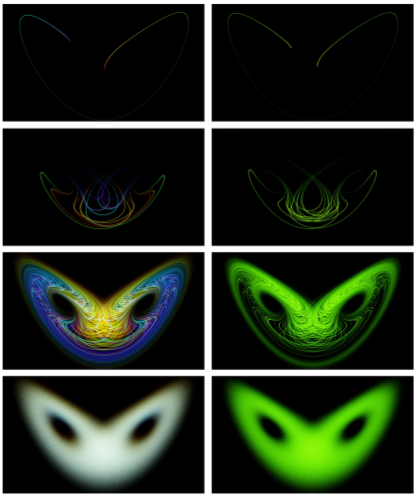
\includegraphics[width=0.48\textwidth]{lz63.png}
  \end{center}
  \caption{Snapshots of Lorenz 63. Left side varying $\rho$ and right side varying the initial conditions. Their respective times are 1.67, 5.0, 10.0 and 41.67.}
  \label{fig:lz63}
\end{wrapfigure}
$u_0 = (12.00, 6.82, 36.47)$. Here $\rho$ is uniformly distributed on the interval $[27,29]$. A smaller $\rho$ is indicated by colors with shorter wavelenghts, smaller is indicated by blue, larger by red. On the right column, they plot snapshots of the same number of trajectories with the same density $\rho = 28$, but with a varying initial condition. Such conditions are characterized by vectors uniformly distributed along $u_0 \pm \Delta u_0$, where $\Delta u_0 = [0.0939,-0.001053,1.05]$\footnote{Those numbers come from the NILSS solution}. Later they will see that $\Delta u_0$ is chosen to have similar effects to the trasient effect of varying $\rho$.

There are many similarities and small differences between the effects observed when $\rho$ is varying and when the initial conditions $u_0$ are changed. As we can see on the first three rows of Fig. \ref{fig:lz63}, in the sorth time, changing $\rho$ results in diverging trajectories which look like the effect of only varying $u_0$: we call this the transient effect\footnote{Read more about this effect, it looks interesting.}.

The picture on the last row of Fig. \ref{fig:lz63} is obtained after letting trajectories evolve for a long time. The picture on the left, has a similar shape as the atractor on the right. However the picture on the left is a superposition of many attractors with different parameters, and if we take a closer look, we can see that it actually has different colors on certain parts (for example on the top). The red color on the upper rim, and the blue on the lowe, indicates that as $\rho$ increases, the attractor moves upward. As a conclussion, varying $\rho$ results in a shifted attractor: and they call this the long-time effect\footnote{Long-time effect: the attractor shifts as $\rho$ changes.}.

the long-time effect generated from vrying $\rho$ is important for computing the long-time sensitivity, however, it is hidden on diverging trajectories and it can only be appreciated after a long time and an ensemble of millions of trajectories. As noted before, the transient effect is reflected by diverging trajectories, hence, if we can find two non-diverging trajectories, one with $\rho$ and the other with $\rho+\Delta \rho$ then their difference will not contain the transient effect. And therefore their difference will only have the long-time effect\footnote{What do we understand from ``non-diverging"?}.

The main goal of the paper is then to devise a method able to generate the transient effect and then take it away from a varying $\rho$, so that we can find trajectories that do not diverge from one another, and whose difference contains only the long-time effect. As a matter of fact, in Fig. \ref{fig:lz63}, $\Delta u_0 = v\Delta p$ and $v$ represents the NILSS solution. As they show aveltually, this change in the initial conditions yields the transient effect, an by subtracting it from the two effects of a varying $\rho$, we can obtain the long-time effect using a short trajectory.

\section{The idea of tangent NILSS}

To strenghten up the ideas developed in the last section, in Section \ref{3.1}, the two perturbations are characterized mathematically as two different tangent solutions, i.e. inhomogeneous and homogeneous tangents. To get the long-time effect $v$ (inhomogeneous tangent), we construct an homogeneous tangent $w$ representing the long-time effect, and sustract it from the conventional inhomogeneous one $v^*$. Both effects are included in $v^*$. In Section \ref{3.2} is shown how to construct $w$ as a linear combination of unstable Characteristic Lyapunov Vectors (CLV). In Section \ref{3.3} they give an efficient way to compute $w$ from $v^*$ and a bunch of homogeneous solutions. And finally, our goal, in Section \ref{3.4} they show how to compute $d\langle J \rangle_\infty /ds$.

\subsection{Describing perturbations by tangents}\label{3.1}

Now we use tangent solutions to describe trajectory perturbations coming from perturbations on the initial data and parameters. The perturbation due to parameter changes is described by inhomogeneous tangents\footnote{I don't know why}, and the one due to intial data changes is described by homogeneous tangents.

First we, differentiate Eq. \ref{eq:1} with respect to $s$, keeping $\phi$ constant. And rename $v^* = \partial u/ \partial s$. Thus, the equation for $v^*$ can be obtained from:
\begin{eqnarray}
  \frac{d}{ds} \left( \frac{du}{dt} \right)  = \frac{\partial }{\partial s} \left( \frac{\partial u}{\partial t} \right)= \frac{d}{ds}f(u,s),\nonumber\\
  \frac{\partial }{\partial t} \left( \frac{\partial u}{\partial s} \right) = \frac{\partial f}{\partial u} \frac{\partial u}{\partial s} + \frac{\partial f}{\partial s}\cancelto{1}{\frac{\partial u}{\partial u}},\nonumber\\
  \frac{\partial v^*}{\partial t}  = \partial_u fv^* + \partial_s f,
  \label{des:1}
\end{eqnarray}
For this to be true we need $u\in C^2$ at least. The initial conditions are easier to differentiate, since $\phi$ is fixed
\begin{eqnarray}
  \frac{d}{ds} u(t=0) = \cancelto{0}{\frac{d u_0(\phi)}{ds}},\nonumber\\
  v^*(t=0) = 0.\label{des:2}
\end{eqnarray}
Therefore, using Eqs. \ref{des:1} and \ref{des:2}, the dynamical equation for $v^*$ is
\begin{equation}
  \frac{dv^*}{dt} + \partial_u fv^* = \partial_s f, \quad v^*(t=0) = 0
  \label{eq:4}
,\end{equation}
where $\partial_u f$ is an $\mathbb{R}^m\times\mathbb{R}^m$ matrix\footnote{Think about why is m.} and $\partial_sf$ is an $\mathbb{R}^m$ vector. We must notice two things here: First, the second equation reflects that $u_0$ remains unchanged (the initial conditions). Second, by definition $v^*$ reflects the trajectory perturbation due to changes on the parameters, keeping the initial data constant, this was shown in the first column of Fig. \ref{fig:lz63}.

Under the assumption of ergodicity, the initial conditions don't affect the long-time behaviour. This suggests that $\phi$ is not necesarily fixed if we are only interested in the change of a long-time average. So, we define inhomogeneous tangent solutions as solutions to Eq. \ref{eq:4} without the initial condition,
\begin{equation}
  \frac{dv}{dt} + \partial_u fv = \partial_s f.
  \label{eq:5}
\end{equation}

Now, we got rid of the initial condition, so the system is underdetermined. In order to have a well-posed problem again we can add initial conditions or add one more equation. The second will be our approach. By definition $v$ reflects the perturbation of the trajectory due to a change in the parameter. That was half of what we were looking for, the other half is the part that describes perturbations on the trajectory due to changes in the initial data.

We define $w = \partial u / \partial \phi$, where $s$ is fixed and $w$ satisfies the so called homogenenous tangent equation:
\begin{equation}
  \frac{dw}{dt} + \partial_u fw = 0.
  \label{eq:6}
\end{equation}
By it's definition, $w$ describes the divergence in trajectories due to changes on the initial conditions while $s$ is fixed. As shown on the right column of Fig \ref{fig:lz63}.

Hence $v^*$ and $w$ describe the effects of only varying $s$ and $\phi$ respectively. for two different inhomogeneous solutions $v^*$ and $v$ the difference between them is a homogeneous tangent solution\footnote{We can go from $v^*$ to $v$ by adding the right $w$ to $v^*$, this will work, since $w$ is solution to the homogeneous equation and is equivalent to add one zero on the left hand side.}.

We know that by changing $s$ we generate two effects: one is equivalent to change $u_0$, and the other shifts the attractor. We are interested on the second one, so we need to find $w$ such that $v = v^* + w$ contains only the long-time effect.

Naturally we can not only add but also subtract $w$ from $v^*$. Such subtraction is the main idea behind NILSS. As previously stated, we want to find two trajectories associated with parameters $s$ and $s + \Delta s$ that do not diverge from each other. We can say that $v$ is sufficient to reveal the long time effect of varying one parameter, if the euclidean norm of its orthonormal projection onto $V^\perp (u)$ remains bounded as the trajectory length goes to infinity. We denote this sufficient v by the shadowing direction $v^\infty$, whose existence is proved by the shadowing Lemma\footnote{Read about this.}. Here $V^\perp(u)$ is defined as:
\begin{equation}
  V^\perp(u) = \{ p\in \mathbb{R}^m  : p^T f(u) = 0 \}.
  \label{eq:7}
\end{equation}
Moreover the orthogonal projection $p^\perp$ of $p$ is defined as:
\begin{equation}
  p^\perp = p - \frac{f^T p}{f^Tf}f.
  \label{eq:8}
\end{equation}
$v^{\infty\perp}$ is defined by substituting $p$ by $v^\infty$. We define $w^\perp$, $\delta u ^\perp$, $v^{*\perp}$, and ${\zeta_j^\perp}$ in a similar way. We use the norm of $v^{\infty\perp}$ because it describes the perpendicular distance between two trajectories.
\subsection{Constructing $w$ from unstable Characteristic Lyapunov Vectors (CLV)}\label{3.2}

The main goal of NILSS is to find a $w$ such that $v^\perp = v^{*\perp} + w^\perp$ approximates $v^{\infty \perp}$ on a finite trajectory. $v^\infty$ is the inhomogeneous tangent, whose projection $v^{\infty\perp}$ remains bounded. It is, nevertheless, important to notice that $v^\perp$ can be unbounded for infinite long trajectories. But don't worry, we work on finite trajectories with NILSS, and on those trajectories $v^\perp$ is a good approximation\footnote{This is not so obvious to me now.} of $v^{\infty\perp}$. This means that when computing sensitivities, using $v^\perp$ yields similar results as using $v^{\infty\perp}$.

In this subsection, one way to construct $w$ is shown, suposing we know $v^\infty$ and all the CLV\footnote{Read about CLV.}. We wouldn't use this in practice, since it is really expensive, but it is a good way to show that we only need a linear combination of unstable CLV to construct $w$. And using this knowledge NILSS will be developed in the next subsection.

We need the definitions of Lyapunov Exponent (LE) and the corresponding CLVs. Moreover, we assume the system has a full\footnote{What does it mean full here?} set of LEs and CLVs, i.e. $\exists$ $ \{\lambda_j, j=1,2,\ldots,m\}$ such that for every trajectory on the attractor, there is a unique representation of the homogeneous tangent solution $w(u)$:
\begin{equation}
  w(u) = \sum_{j=1}^m a_j\zeta_j(u),
  \label{eq:9}
\end{equation}
where $a_j\in \mathbb{R}$ remains constant throughout the trajectory.

Each $\zeta_j(u)$ is a homogeneous tangent solution, and its norm behaves exponentially on time, i.e. $\exists C_1, C_2 > 0$ s.t. $\forall u(t), j, t$, it satisfies
\begin{equation}
  C_1 e^{\lambda_jt}\norm{\zeta_j(u(0))} \leq \norm{\zeta_j(u(t))} \leq C_2 e^{\lambda_jt}\norm{\zeta_j(u(0))},
  \label{eq:10}
\end{equation}
where $\{\lambda_j\}$ and $\{\zeta_j\}$ are LEs and CLVs, respectively. CLVs with $\lambda_j>0$ are called unstable modes, CLVs with $\lambda_j<0$ stable, and those with $\lambda_j=0$ neutral. We will denote unstable modes by $\lambda_1,\ldots,\lambda_{m_{us}}$ and the neutral modes by $\lambda_m$. The rest will be the stable modes\footnote{Here we can see why unstable modes are called like this. Basically the positive factor of the exponential makes the CLVs grow over time.}.

We assume that for all $s$ we are interested in there is no point $u$ on the attractor $\Lambda$ such that $f(u)=0$ and $\Lambda$ is bounded. These two assumptions imply that such mode is neutral, i.e. the LE of the CLV is 0. We also assume that $f(u)$ is the only neutral mode.

The CLVs are not necessarily in $V^\perp$, but we can project them, and then Eq. \ref{eq:9} becomes:
\begin{equation}
  w^\perp(u) = \sum_{j=1}^{m-1} a_j\zeta_j^\perp(u),
  \label{eq:11}
\end{equation}
Because $V^\perp$ is perpendicular to $f(u)$, the projection of the neutral mode is zero\footnote{It is easy to see this if we substitute $\zeta_j^\perp = 0$ in Eq. \ref{eq:8}.}. This means that in Eq. \ref{eq:11} only the unstable and stable modes are taken on the sum, and since we have only one neutral mode the remaining modes are $m-1$. We use also the LEs to classify the projections of the CLVs as stable and unstable.

We assume all CLVs are bounded from each other\footnote{What does this means?}. Under this assumption, the norm of stable and unstable modes ${\zeta_j^\perp}$ also behaves like exponentials, as defined in Eq. \ref{eq:10}.

Now let's suppose we know $v^\infty$ and all its CLVs. Since $v^\infty - v^*$ is a homogeneous tangent solution, we can decompose $v^{\infty \perp} - v^{*\perp}$ using Eq. \ref{eq:11}. By using the first $m_{us}$ coefficients we let
\begin{equation}
  w= \sum_{j=1}^{m_{us}} a_j \zeta_j.
  \label{eq:12}
\end{equation}
Therefore $v^\perp = v^{*\perp} - w$ approximates $v^{\infty\perp}$, since $v^{\infty\perp} - v^\perp$ contains only stable modes, and they decay exponentially with time.

As we said before, in practice this is not implemented since it requires the knowledge of $v^\infty$ and all its CLVs. But the lesson we will carry onto the next section is this one: $w$ is a linear combination of only unstable modes.
\subsection{Computing $v^\perp$ by NILSS}\label{3.3}
In NILSS we compute $v = v^* + w$ such that $v^{\perp} \approx v^{\infty \perp}$. We want the integration of $v^{\perp}$ to approximate the one of $v^{\infty \perp}$ and later use $v^{\perp}$ to compute the sensitivity. To do this, we solve the NILSS problem on a time interval, this problem is to minimize the $L^2$ norm of $v^\perp = v^{*\perp} + W^\perp a$:
\begin{equation}
  \min_a \frac{1}{2} \int_0^T (v^{*\perp} + W^\perp a)^T (v^{*\perp} + W^\perp a) dt,
  \label{eq:13}
\end{equation}
which is a least squares problem with arguments $a\in \mathbb{R}^M$, where $M$ is an integer larger\footnote{Why larger} than the number of positive LEs $m_{us}$. $v^*$ is the conventional tangent solution, and $W^\perp (t)$ is a matrix whose columns are homogeneous tangent solutions $\{w_j^\perp(t), j=1,\ldots,M\}$. The initial conditions $\{w_j^\perp(0) $ are randomized unit vectors in $\mathbb{R}$.

\begin{wrapfigure}{l}{0.3\textwidth} % Inline image example
  \begin{center}
    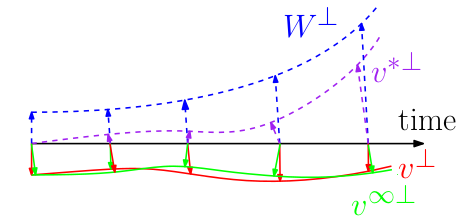
\includegraphics[width=0.28\textwidth]{diff.png}
  \end{center}
  \caption{Intuition of NILSS.}
  \label{fig:2}
\end{wrapfigure}

Now we need to make sure that $v^\perp$ exists, but we saw that we can construct it using unstable CLVs instead of $W$. Furthermore, it has been proven\footnote{Need to check the reference.} that as times evolves, the span of $\{w_j^\perp(t), j=1,\ldots,M\}$ converges to the span of CLVs $\{\zeta_j^\perp(t), j=1,\ldots,M\}$ with the largest $M$ LEs. So, if we replace $W$ by the CLVs we span a similar space, and the solution, as we know lies on such space\footnote{This is really important, it should be on the slides.}.

Next, we need to understand why minimizing the $L^2$ norm of $v^{*\perp} + W^\perp a$ yields $v^\perp \approx v^{\infty\perp}$. First, $v^\perp$ can be written as the summation of $v^{\infty \perp}$ and some homogeneous tangents\footnote{I'm not pretty sure why. Maybe it's a consequence of $v^\perp\approx v^{\infty\perp}$}. Because $v^{\infty\perp}$ is bounded and the unstable modes grow exponentially, then minimizing $v^\perp$ over a long trajectory implies the difference $v^\perp - v^{\infty\perp}$
cannot contain a significant amount of unstable modes. Although stable modes may be left in the difference, they will decay exponentially. This effect is shown on Fig. \ref{fig:2}

\subsection{Computing $d\langle J \rangle_\infty /ds$ from the tangent solution}\label{3.4}
Since $v-v^\perp$ is parallel to f\footnote{How do we know that? Moreover, can we just multiply a constant to go from one to the other?}, we can define $\xi$ as the scalar that fulfills:
\begin{equation}
  \xi f = v - v^\perp
  \label{eq:14}
\end{equation}
To find a pair $(v^\perp,\xi)$, we first find a $v$ that solves Eq. \ref{eq:5}, project v onto the subspace $V^\perp$ to find $v^\perp$, then use Eq. \ref{eq:14} to find $\xi$.

once we have the solution vector $a$ of NILSS, we can construct $v=v^{*} + Wa$ and compute the corresponding $\xi$. And then we have the following approximation for $d\langle J \rangle_\infty / ds$
\begin{equation}
  \frac{d\langle J \rangle_\infty}{ds} \approx \frac{1}{T}\left[ \int_0^T (\partial_u Jv + \partial_s J)dt + \xi|_0^T \langle J \rangle_T - (\xi J)|_0^T\right],
  \label{eq:15}
\end{equation}
Notice that in Eq. \ref{eq:15}, the tangent solution $v$ is used intead of its projection $v^\perp$. This equation is later derived here.
\subsection{Benefits of NILSS}\label{3.5}
the first benefit is that it is easily implemented with existing tangent solvers\footnote{Remains to be seen.}. The data used in the NILSS problem are $v^{*\perp}$ and $\{ w_j^\perp \}$. $v^*$ is the result of a conventional tangent solver\footnote{I still need to read about tangent solvers.}. $\{ w_j \}$ are given by homogeneous tangent solvers, which is just set the right hand side of Eq. \ref{eq:5} equal to zero. Once we obtain those ones, the projections can be done using Eq. \ref{eq:8}.

Another way to get the tangent solutions is to approximate them by finite differences. In this way NILSS requires only primal simulation and no longer the tangent solvers\footnote{Because the tangent solvers were used to obtain the tangent solutions.}.

In NILSS, the computational cost is reduced, since we use only M arguments in Eq. \ref{eq:13}. The main cost is actually the set up, i.e. obtaining $v^{*\perp}$ and $\{ w_j^\perp \}$, hence the computational cost of NILSS is proportional to the number of unstable modes $m_{us}$. Usually we have $m_{us} \ll m$, thus, the cost of NILSS is low.

A nice side-effect is that NILSS uses less memory that LSS. Hence, the tangent solutions of NILSS don't tend to be stored concurrently in memory\footnote{Just read what concurrently means}. NILSS can use tangent solutions stored on external memory, this saves computer memory, but might slow things down.

\section{Tangent NILSS algorithm}

In this section, the stability is controlled by rescaling $v^{*\perp}$ and $W^\perp$ after every short segment of time $\Delta T$. Then we discuss how do we select the number of homogeneous solutions $M$ and the time step $\Delta T$, Finally, we walk through the NILSS algorithm.

\subsection{Solving NILSS on multiple time segments}

Since both $v^{*\perp}$ and $W^\perp$ grow exponentially, we can not ignore the round-off error when storing in the computer. The growht on $v^{*\perp}$ and $W^\perp$ will also generate an ill-conditioned covariance matrix $(w^\perp)^T W^\perp$, since all the $\{w_j^\perp\}$ will eventually be dominated by the fastest growing unstable CLVs. That is why we need reescaling every time step. Here we show how to do it.


\begin{wrapfigure}{l}{0.3\textwidth} % Inline image example
  \begin{center}
    \includegraphics[width=0.28\textwidth]{fig3.png}
  \end{center}
  \caption{Schematization of the reescaling part of the algorithm.}
  \label{fig:3}
\end{wrapfigure}
We make a grid of K+1 points from 0 to $K$. Next the time segment $i$ is defined as $[t_i, t_{i+1}]$. For each time segment $i$, we define an ihnomogeneous solution $\{v_i^*\}$ and homogeneous solutions $\{W_i\}$, such that each $W_i = [w_{i,1},\ldots,w_{i,M}]$. This idea is illustrated in Fig. \ref{fig:3}.

We want to rescale and orthogonalize $v_i^{*\perp}$ and $W_i^\perp$ and the end of every timestep so that they don't become dominated by the fastest growing CLVs. We also want to keep the space $v^{*\perp} + span(W^\perp)$ the same across interfaces, so we have:
\begin{equation}
  v_i^{*\perp}(t_i) + span(W_{i}^\perp(t_i)) = v_{i-1}^{*\perp}(t_i) + span(W_{i-1}^\perp(t_i)).
  \label{eq:16}
\end{equation}

To achieve this, we orthonormalize $W^\perp$ via QR decomposition\footnote{What is a QR decomposition?}:
\begin{equation}
  W_i^\perp(t_{i+1}) = Q_i R_i.
  \label{eq:17}
\end{equation}
We set the initial conditions of the next tangent elements to
\begin{equation}
  W_{i+1}(t_{i+1}) = Q_i.
  \label{eq:18}
\end{equation}
In QR factorization, the column vectors in $Q_i$ and $W_i^\perp$ could represent each other if the column vectors in $W_i^\perp$ are linearly independent. The linear independence of the initial condition of $W_i^\perp$ can be preserved after $\Delta T$ if $f$ is Lipschitz continuous. Hence\footnote{They remain linearly independent, but why would they span the same space?}, the $span(W_i^\perp(t_i)) = span(W_{i+1}^\perp(t_{i}))$.

We subtract from $v^{*\perp}$ it's orthogonal projection on $W^\perp$ to obtain the initial condition of the next timestep:
\begin{equation}
  v^*_{i+1}(t_{i+1}) = v^{*\perp}_i (t_{i+1}) - W_{i+1}^\perp(t_{i+1})b_i,
  \label{eq:19}
\end{equation}
where $b_i = W_{i+1}^\perp(t_{i+1})^T v_i^*(t_{i+1})$. $v_{i+1}^{*\perp}(t_{i+1})$ is still in the space $v_i^{*\perp}(t_i) + span(W_i^\perp(t_i)).$ The norm of $v_i^{*\perp}(t_i)$ is reduced, since it no longer contain the unstable modes that were subtracted through the projection.

We can recover a continuous $v^\perp$ over the whole trakectory. Now Eq. \ref{eq:16} is satisfied, for any $a_{i-1}, \exists a_i$, such that:
\begin{equation}
  v_i^{*\perp}(t_i) + W_i^\perp (t_i)a_i = v_{i-1}^{*\perp}(t_i) + W_{i-1}^\perp(t_i)a_{i-1}.
  \label{eq:20}
\end{equation}
Hence we have the necessary conditions to enforce the continuity requirement:
\begin{equation}
  v_i^\perp(t_i) = v_{i-1}^\perp(t_i).
  \label{eq:21}
\end{equation}
The solution $v^\perp$ over multiple timesteps is equivalent to one over a longer step. However we avoid getting too big CLVs by reescaling every step. Using QR factorization to reescale homogeneous solutions is not a new idea, is widely used for computing LEs\cite{chater}.

\subsection{Determining parameters for NILSS}

In NILSS the user has the posibility of choosing two parameters: the number of homogeneous solutions $M$ to be used and the size of the time-step $\Delta T$. Once both parameters are set we can proceed with our calculations.

The determination of $M$ is made based on the LE. The j-th largest LE $\lambda_j$ is computed by:

\begin{equation}
  \lambda_j \approx \frac{1}{K\Delta T} \sum_{i=1}^L \log{(|d_{ij}|)},
  \label{eq:22}
\end{equation}
where $d_{ij}$ is the j-th diagonal element of $R_i$\footnote{What is $R_i$ and also what is that $K$ in the equation.}. It is important to notice that the computation of ${R_i}$ onlt requires $W$ but not $v^*$, NILSS can compute homogeneous solutions $W$ before $v^*$. While computing $W$ we can gradually increase M and therefore compute more LEs, which appear in decreasing order, until we reach a LE with negative sign, at that point we will know we found all positive LEs.

$\Delta T$ is determined by the constraint that the CLV with the largest LE ($\lambda_1$) does not dominate the M-th LE ($\lambda_M$), then the ratio between the norm of this two satisfies \clearpage
\begin{equation}
  \frac{||\zeta_1^\perp(u(t))||/||\zeta_1^\perp(u(0))||}{||\zeta_M^\perp(u(t))||/||\zeta_M^\perp(u(0))||} \approx \exp((\lambda_1 - \lambda_M)t).
  \label{eq:23}
\end{equation}
As a consequence of this we will have that after a time-step of $t=(\lambda_1 - \lambda_M)^{-1}$ the fastest growing CLV grows about three times larger than the M-th one. If $\Delta T$ is too large then the covariance matrix (it will appear eventually) will be ill conditioned. To prevent this from happening we reescale $W^\perp$ and $v^{*\perp}$ after $\Delta T < (\lambda_1 - \lambda_M)^{-1}$. On the other hand, if $\Delta T$ becomes very small then this will lead to a larger optimization problem, and more steps. This will give the criteria for the lower bound.

Both criteria are \textit{a posteriori}, which means that we actually need to run  NILSS for a few segments to check if they are satisfied. In most cases choosing a small $\Delta T$ does not contribute significantly to the computational cost of the algorithm, so the recomendation is to actually seting small $\Delta T$ to begin with and then modify it according to the given criteria. After $\Delta T$ is chosen we can determine $M$ accordingly.

\subsection{Pre-processing}

First, we integrate the primal problem over a sufficient period of time until it lands on the attractor, at that point we can set $t=0$ and begin the calculations from $t=0$ to $t=T$ to obtain the primal solution.

\subsection{Computing the homogeneous solution $\{W_i\}$}

We compute one inhomogeneous and M homogeneous tangent equations for each of the $K$ time segments $[t_0,t_1],\ldots,[t_K-1, t_K]$, where $t_0 = 0$ and $t_K = T$.

We start at the first segment with random initial conditions for each column vector in $W$:
\begin{equation}
  W_0 (0) = [w_{0,1},\ldots,w_{0,M} ], \quad \textnormal{with }\quad w_{0,j}\in V^\perp(u(0)).
  \label{eq:24}
\end{equation}
Then, we proceed with the following algorithm, wich starts at $i=0$.
\section{Questions}
\begin{description}
  \item [1] What is a tangent solution?
  \item [2] What is a least squares problem?
  \item [4] What are the Lorenz 63 and the CFD simulation of flow over backward-facing step systems?
  \item [5] Why is NILSS good for systems with may degrees of freedom and few unstable modes?
\end{description}
\newpage
\section{To do}

\begin{enumerate}
  \item Find what tangent solutions are.
  \item Explain how the final solution is used to compute sensitivities.
\end{enumerate}



\bibliography{MyNotes.bib}
\bibliographystyle{ieeetr}
%
% Example citation \cite{Figueredo:2009dg}.
%
% %------------------------------------------------
%
% \subsection{Subsection 1} % Sub-section
%
% \lipsum[1] % Dummy text
%
% %------------------------------------------------
%
% \subsection{Subsection 2} % Sub-section
%
% \lipsum[2] % Dummy text
%
% %------------------------------------------------
%
% \subsubsection{Subsubsection 1} % Sub-sub-section
%
% \lipsum[3] % Dummy text
%
% \begin{figure}[H] % Example image
% \center{\includegraphics[width=0.5\linewidth]{placeholder}}
% \caption{Example image.}
% \label{fig:speciation}
% \end{figure}
%
% %------------------------------------------------
%
% \subsubsection{Subsubsection 2} % Sub-sub-section
%
% \lipsum[4] % Dummy text
%
% %----------------------------------------------------------------------------------------
% %	MAJOR SECTION 1
% %----------------------------------------------------------------------------------------
%
% \section{Content Section} % Major section
%
% \lipsum[5] % Dummy text
%
% %------------------------------------------------
%
% \subsection{Subsection 1} % Sub-section
%
% \subsubsection{Subsubsection 1} % Sub-sub-section
%
% \lipsum[6] % Dummy text
%
% %------------------------------------------------
% \newpage
% \subsubsection{Subsubsection 2} % Sub-sub-section
%
% \lipsum[6] % Dummy text
% \begin{wrapfigure}{l}{0.4\textwidth} % Inline image example
%   \begin{center}
%     \includegraphics[width=0.38\textwidth]{fish}
%   \end{center}
%   \caption{Fish}
% \end{wrapfigure}
% \lipsum[7-8] % Dummy text
%
% %------------------------------------------------
%
% \subsubsection{Subsubsection 3} % Sub-sub-section
%
% \begin{description} % Numbered list example
%
% \item[First] \hfill \\
% \lipsum[9] % Dummy text
%
% \item[Second] \hfill \\
% \lipsum[10] % Dummy text
%
% \item[Third] \hfill \\
% \lipsum[11] % Dummy text
%
% \end{description}
%
% %----------------------------------------------------------------------------------------
% %	MAJOR SECTION X - TEMPLATE - UNCOMMENT AND FILL IN
% %----------------------------------------------------------------------------------------
%
% %\section{Content Section}
%
% %\subsection{Subsection 1} % Sub-section
%
% % Content
%
% %------------------------------------------------
%
% %\subsection{Subsection 2} % Sub-section
%
% % Content
%
% %----------------------------------------------------------------------------------------
% %	CONCLUSION
% %----------------------------------------------------------------------------------------
%
% \section{Conclusion} % Major section
%
% \lipsum[12-13]

%----------------------------------------------------------------------------------------
%	BIBLIOGRAPHY
%----------------------------------------------------------------------------------------

%\begin{thebibliography}{99} % Bibliography - this is intentionally simple in this template
%
% \bibitem[Figueredo and Wolf, 2009]{Figueredo:2009dg}
% Figueredo, A.~J. and Wolf, P. S.~A. (2009).
% \newblock Assortative pairing and life history strategy - a cross-cultural
%   study.
% \newblock {\em Human Nature}, 20:317--330.
%
% \end{thebibliography}

%----------------------------------------------------------------------------------------

\end{document}
